\documentclass[../report.tex]{subfiles}

\begin{document}
\section{State Machine Patterns}
State Pattern er et af de 23 GoF patterns. Det hører til kategorien Behavioral Patterns, fordi den definerer måden man kontrollerer kommunikationen mellem klasserne. State Pattern bliver brugt tilm at ændre adfærd på et objekt, når dets interne state bliver ændret.
\\

State Pattern et objekts klasser til, at ændre ved run-time, uden at ændre interfacet der bruges til, at tilgå objektet, eller tabe den nuværende state. Man bruger en context til at skjule ændringerne.

\begin{figure}[H]
    \centering
    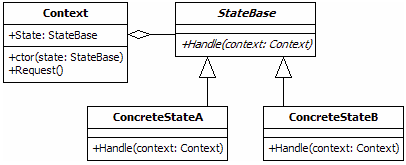
\includegraphics{pics/state_pattern.PNG}
    \caption{State Pattern}
    \label{fig:state_pattern}
\end{figure}

\begin{table}[H]
    \centering
    \begin{tabular}{l|p{0.7\textwidth}}
        Klasse          & Beskrivelse        \\ \toprule
        Context                & Denne klasse bliver brugt af klienter af state design pattern. Klienter har ikke adgang til state objekterne direkte. Til enhver tid vil Context klassen holde et konkret state objekt, der kun fortæller om den nuværende state. Den består også af aktioner hvilket skal udføres alt efter hvilken state den modtager.    \\ \midrule
        Statebase &: Er den abstrakte klassen og base klassen for de konkrete klasser (subklasser). Statebase definerer grænsefladen, som bliver brugt af context objekt til, at tilgå den skiftelige funktionalitet. Den består typisk af default implementeringer af alle handlers.        \\ \midrule
        SubklasserneA/B    & Består af de rigtige funktionaliteter der bliver brugt af context objektet. Hver state klasse har en adfærd, der er gældende til en enkelt state af context objektet. De kan også bestå af instruktioner, der sørger for at context skifter state. \\ \bottomrule
    \end{tabular}
    \caption{sammenligning af WPF og UWP}\label{tab:wpfVSuwp}
\end{table}

\subsection{Sammenligning: Switch/Case-implementering med GoF State}

\begin{figure}[H]
    \centering
    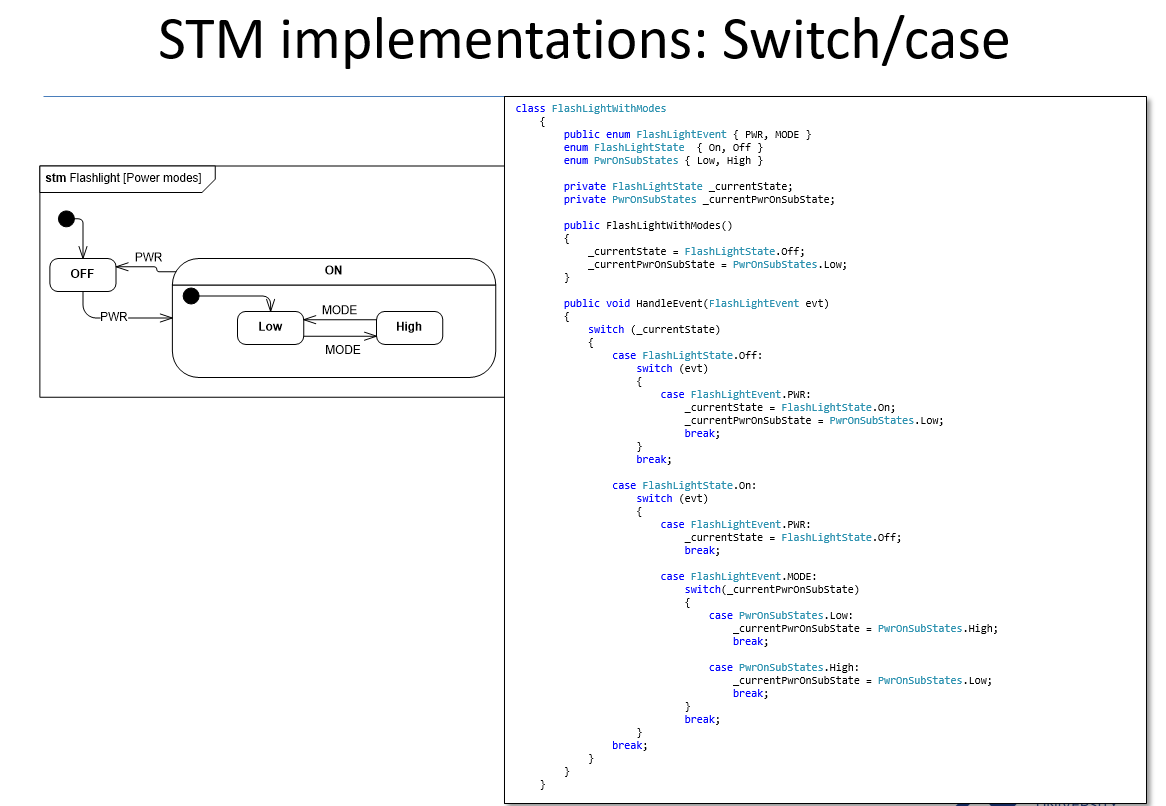
\includegraphics[width = \textwidth]{pics/STM_impl_switch_case.PNG}
    \caption{STM Switch/Case}
    \label{fig:stm_switch_case}
\end{figure}

\subsection{The GoF State}
\begin{figure}[H]
    \centering
    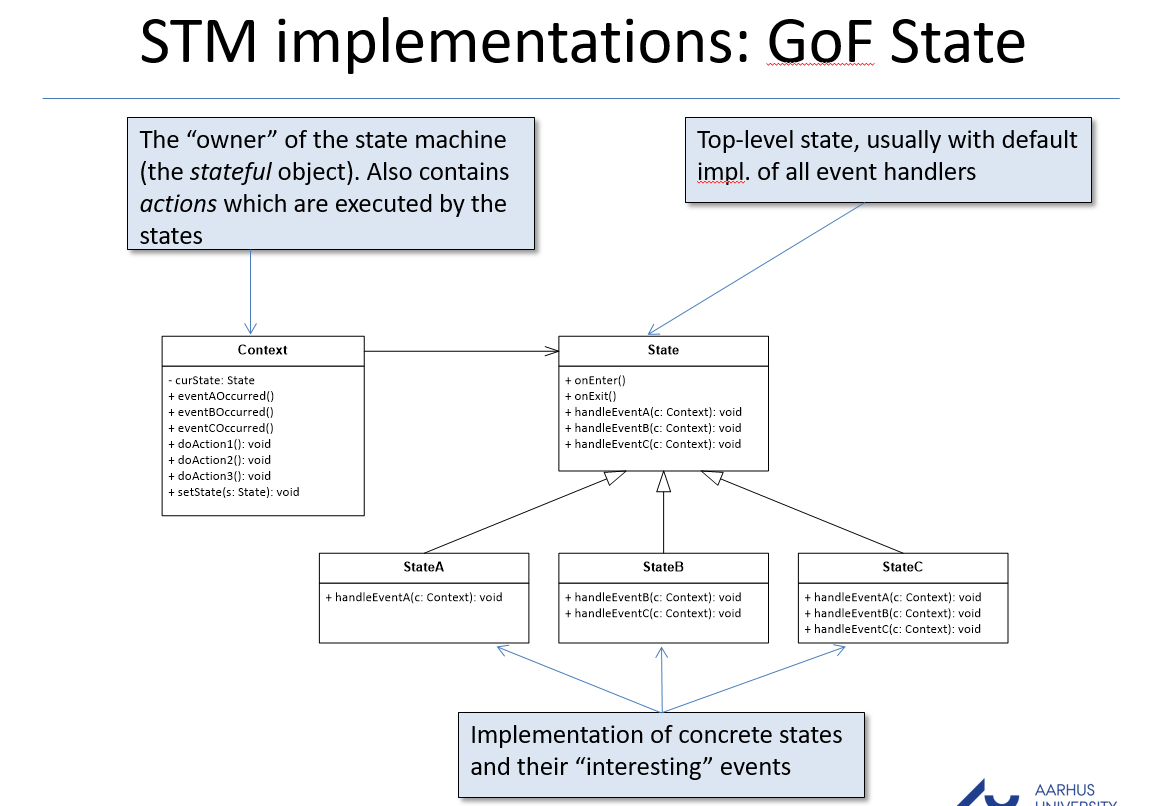
\includegraphics[width = \textwidth]{pics/stm_state_gof.PNG}
    \caption{STM Switch/Case}
    \label{fig:stm_state_gof}
\end{figure}

Når man arbejder med switch cases kan de bliver meget komplekse, når systemet bliver for stort. Dette skyldes, at det kan forekomme mange states inkl. Nested states. Derfor anvendes GoF. Me der vil altid være fordele og ulempter

\subsubsection*{Fordele}
\begin{itemize}
    \item Let at udvide med nye states ved at tilføje et objekt (OCP)
    \item Let at sikre at alle metoder bliver udført i de forskellige states da den abstrakte base klasse definerer de metoder.
    \item Let at udvide en states adfærd ved nedarvning fra staten.
\end{itemize}

\subsubsection{Ulemper}
\begin{itemize}
    \item Kode kompleksiteten bliver høj
    \item Svære at se relationerne mellem klasserne, da de er spredt mellem flere forskellige klasser end i switch.
\end{itemize}
\end{document}
